\problemname{Currents}

Well-hidden in the atrium of an abandoned house, you have found an ancient book that uncovers the most well-kept secret of the city of Bonn.
Deep below the city, there is a system of $N$ caves, connected by $M$ water channels.
Within each water channel there's a one-directional magical current that can quickly transport a boat along the channel.
The cave system currently has exactly one exit that is located in cave $N-1$.

You are very excited about your discovery and cannot wait to explore the caves! 
However, the cave system is inhabited by a troll who likes to have some fun with uninvited visitors. 
The troll has some limited magical power – which he can use \textbf{at most once} during your visit – to modify the cave system and make it harder for you to reach the exit.

Your visit to the cave system will consist of a sequence of rounds. Each round will be as follows:

\begin{enumerate}
\item First, the troll gets to choose whether or not he uses his magical power. If he does, his spell does all of the following:
	 \begin{itemize}
\item reverses the direction of the magical current in every channel: $a \rightarrow b$ will change to $b \rightarrow a$ immediately;
\item closes the exit in cave $N-1$; and
\item opens a new exit in cave $0$.
\end{itemize}
\item Then, you choose a magical current that flows from your present cave, and use your boat to travel to another cave. For simplicity, we will call the use of a boat a ``move''.
\end{enumerate}

Additionally, whenever you are in the same cave as the exit, you will \textbf{immediately} use it to leave the cave system. Note that this can even happen during a round if you are in cave $0$ and the troll decides to use his magical power.

Your goal is to leave the cave system as quickly as possible to be in time for the closing ceremony of the EGOI.
The troll's goal is exactly the opposite; he wants to keep you in his caves for as long as possible.
The troll always knows your location and he will pick the moment at which to use his magical power in a way that serves his goal the best.

Separately for each cave $c$ ($0 \leq c \leq N-2$) consider the scenario in which you start in cave $c$. For each of these scenarios, determine the \textbf{smallest number of moves in which you can definitely reach an exit from cave $c$, no matter when the troll chooses to use his power}.

Assuming the spell is not used, every cave is reachable from cave $0$, and cave $N-1$ is reachable from every cave. 

\section*{Input}
The first line of the input contains two integers, $N$ and $M$, where $N$ is the number of caves and $M$ is the number of water channels.
The next $M$ lines of the input each contain two integers, $a_i$ and $b_i$,
representing a channel that right now can be used to travel from cave $a_i$ to cave $b_i$.
There is no channel connecting a cave to itself. For each pair of caves there is at most one channel in each direction.

\section*{Output}
Output a line with $N-1$ integers, where the $i$th integer, $0 \leq i \leq N-2$, is the smallest number of moves within which you can definitely reach an exit if starting from cave $i$.

Note that you do not output the time for cave $N - 1$ (as you would just exit this cave immediately).

\section*{Constraints and Scoring}
\begin{itemize}
\item $2 \leq N \leq 200\,000$.
\item $1 \leq M \leq 500\,000$.
\item $0 \leq a_i, b_i \leq N-1$ and $a_i \neq b_i$.
\item Before the reversal, cave $0$ can reach all caves, and cave $N-1$ can be reached from all caves.
\end{itemize}

Your solution will be tested on a set of test groups, each worth a number of points.
Each test group contains a set of test cases. To get the points for a test group, you need to
solve all test cases in the test group.


\begin{tabular}{|l|l|l|}
  \hline
  Group  &  Score  &  Limits \\
  \hline
   1 & 12 & $M=N-1$, $a_i = i$ and $b_i = i + 1$ for all $i$. In other words, the cave system forms a path $0 \rightarrow 1 \rightarrow 2 \rightarrow \ldots \rightarrow N-1$   \\
  \hline
   2 & 15 & For each $0 \le i \le N-2$, there is a direct channel from cave $i$ to cave $N-1$. Note there can be additional channels.  \\
  \hline
   3 & 20 & $N, M \leq 2\,000$ \\
  \hline
   4 & 29 & After leaving any cave, it is not possible to travel back to it (until the direction reversal). In other words, the channels form a directed acyclic graph.\\
  \hline
   5 & 24 & No additional constraints \\
  \hline
\end{tabular}


\section*{Examples}
For the first sample, consider the case in which you start in cave 
1. Since you do not know when the direction reversal will happen, you should start moving towards the exit at cave 4. You could do that via either cave 2 or cave 3. Going via cave 3 is the better option here since in case the direction reversal happens while you are there, you will now have a channel you can use to travel from cave 3 directly to cave 0 where you'll exit the cave system.

More precisely, there are only three possibilities for when the troll will decide to use his magical power:

\begin{itemize}
\item If the troll uses his power immediately when you're in cave 1, you can then travel from cave 1 directly to cave 0 and exit.
\item If the troll uses his power after you went from cave 1 to cave 3, you can then travel from cave 3 directly to cave 0 and exit.
\item If the troll decides not to use his power in either of those two situations, you will travel from cave 3 to cave 4 and exit.
\end{itemize}

In the first option you only had to make one move, in each of the other options you made two moves. This means the answer for this case is $\max(1,2,2) = 2$.

Note that if you choose to go from cave 1 to cave 2, the troll can force you to make three moves.

\begin{figure}
\centering
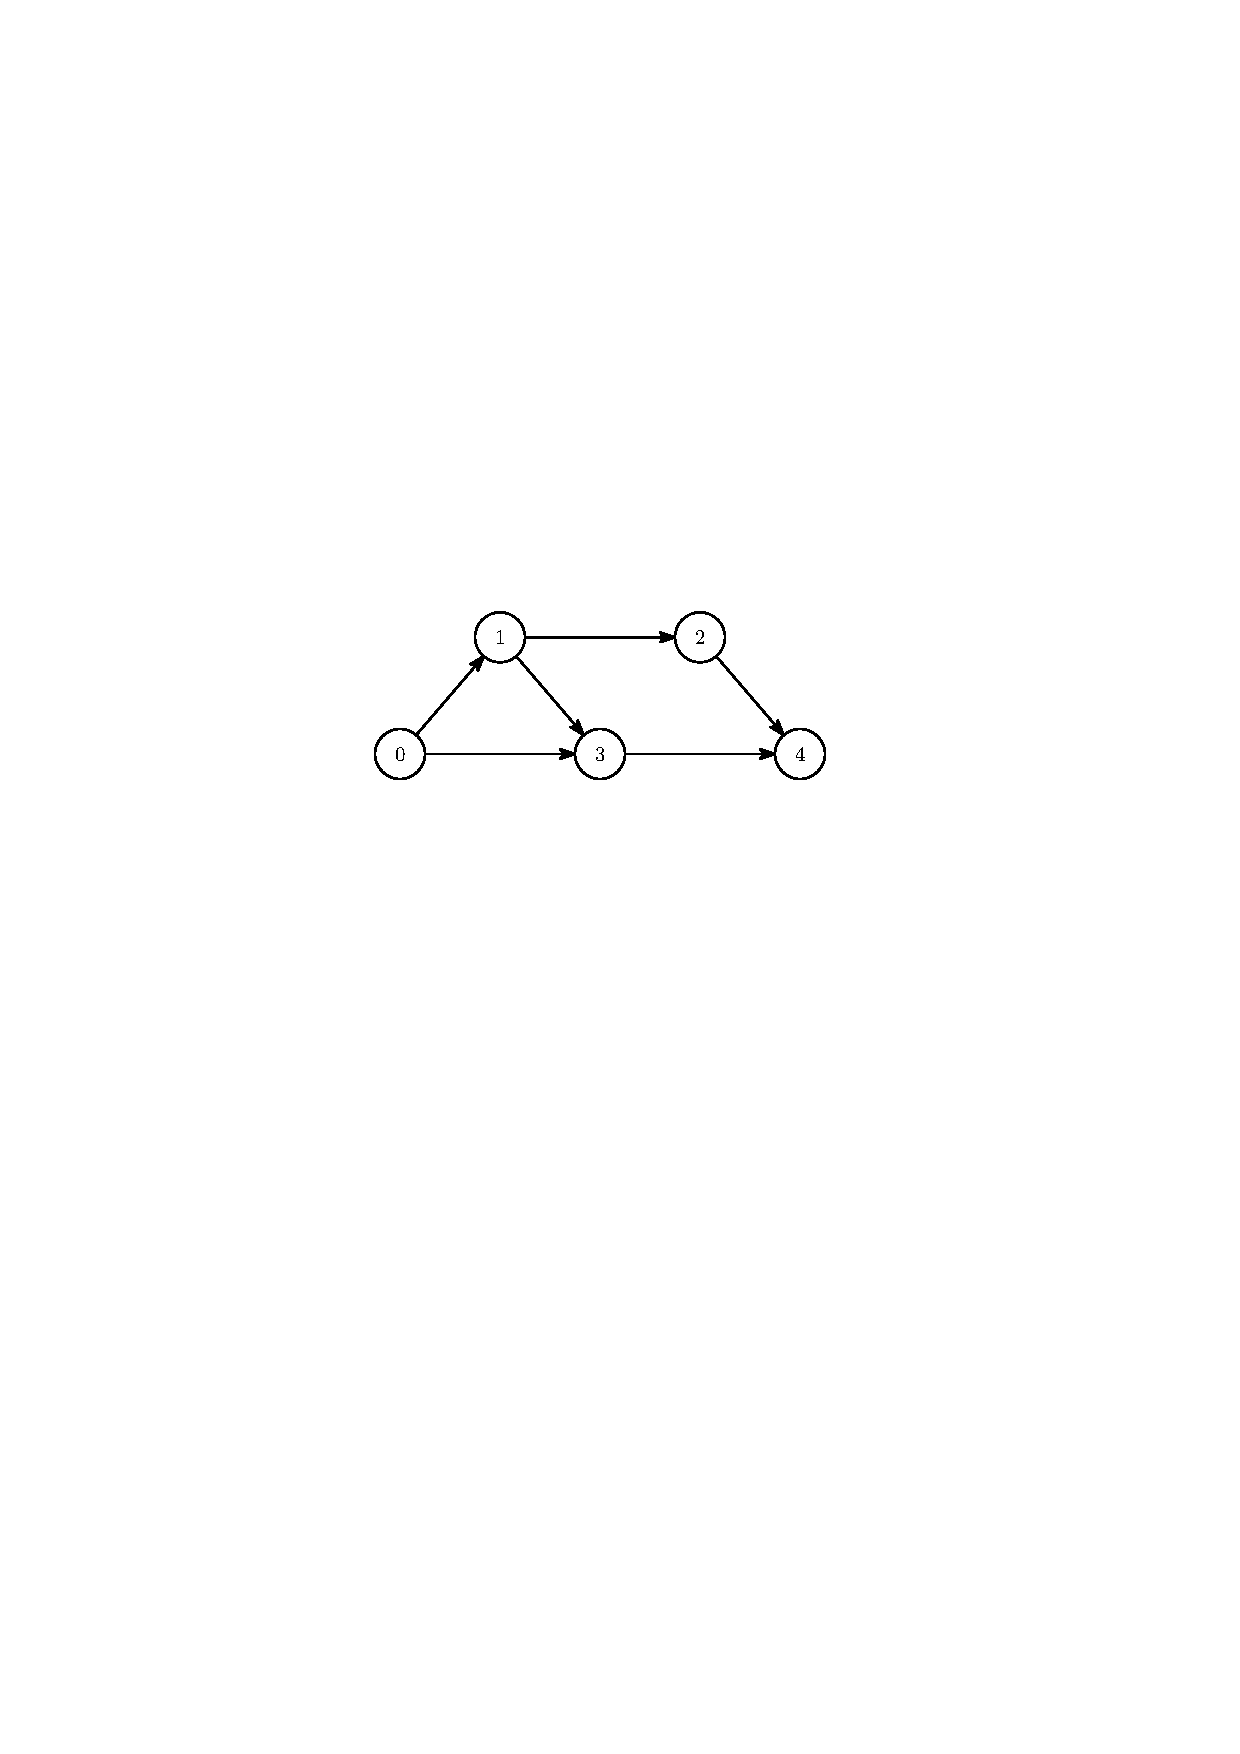
\includegraphics[width=0.8\textwidth]{sample-1}
\end{figure}

The first and second samples satisfy the constraints of test groups 3, 4 and 5.
The third sample satisfies the constraints of all test groups.
The fourth sample satisfies the constraints of test groups 3 and 5, and is illustrated below.

\begin{figure}
\centering
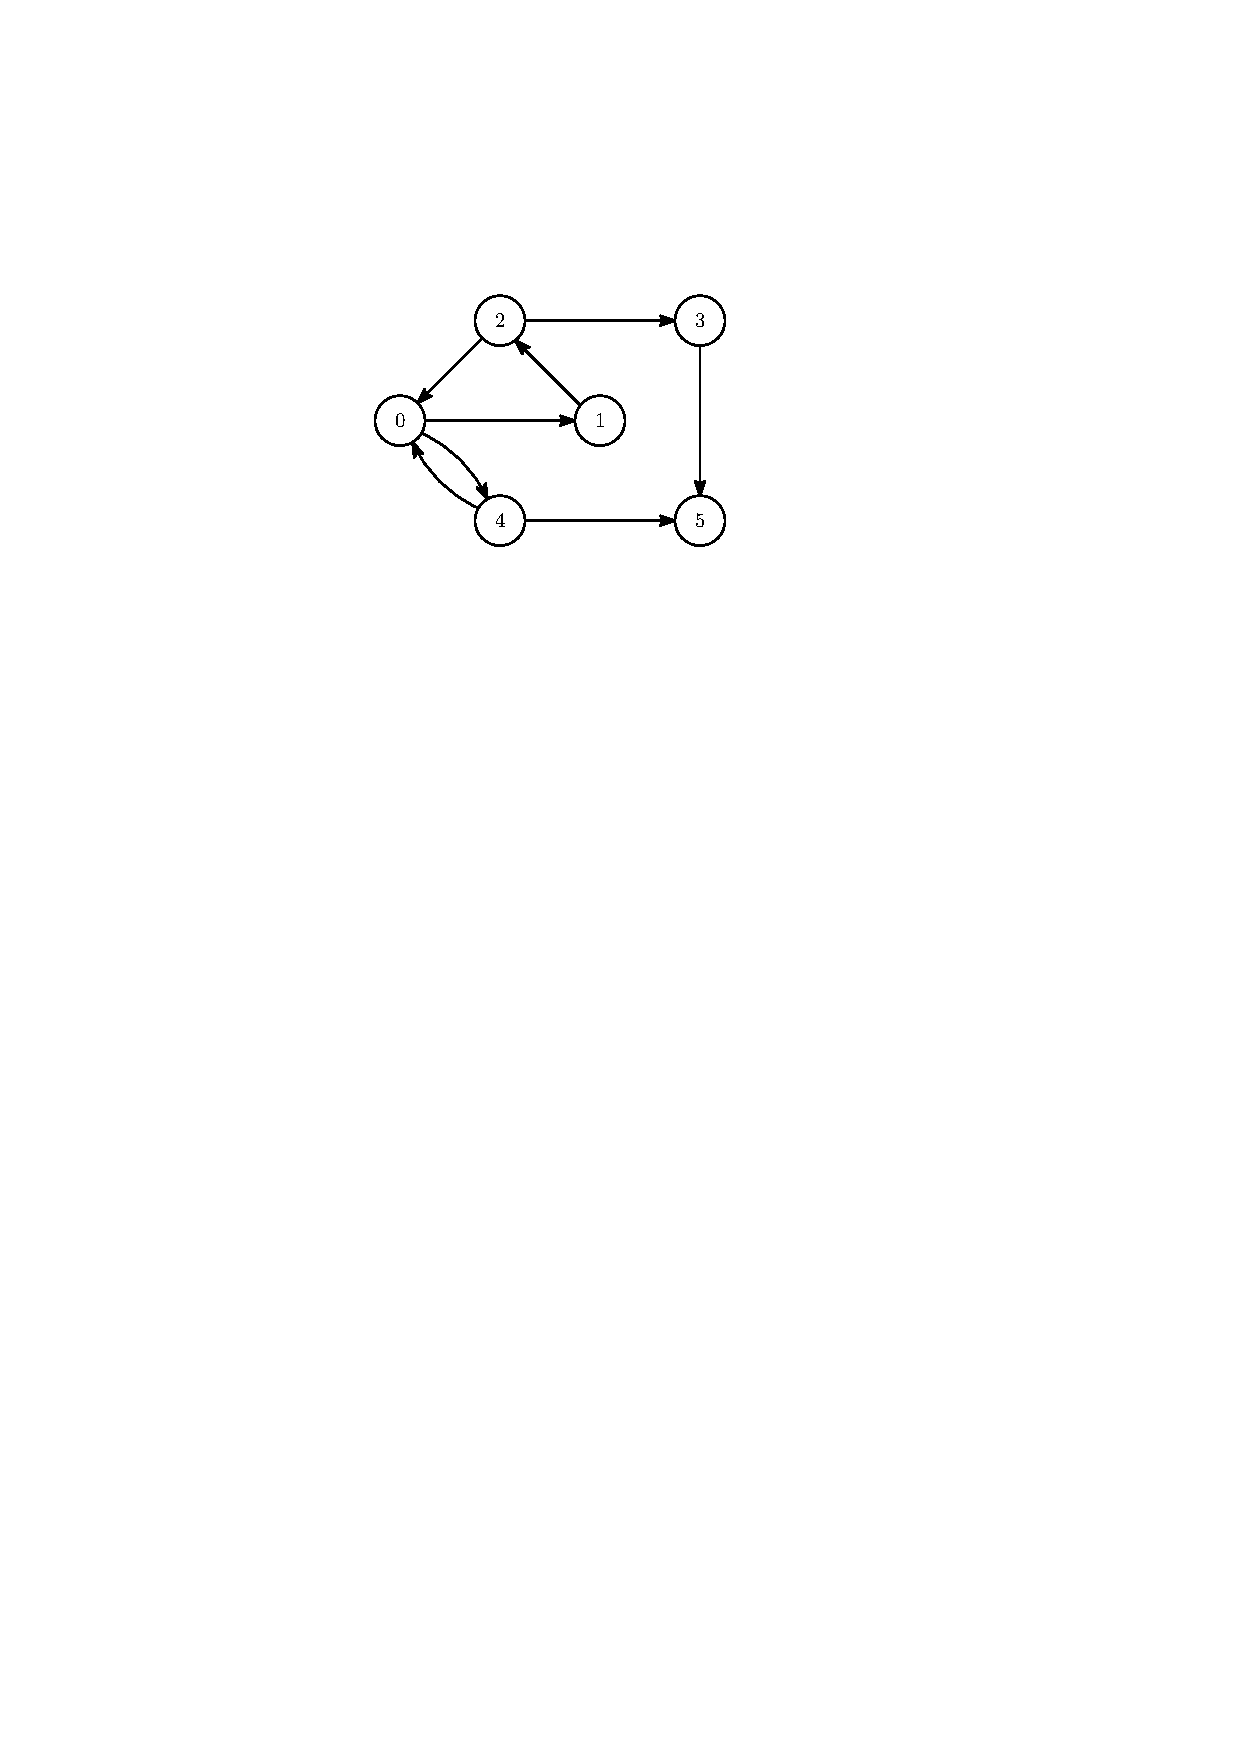
\includegraphics[width=0.8\textwidth]{sample-2}
\end{figure}

